%Texlive-full Version 3.141592-1.40.3 (Web2C 7.5.6)
%Kile Version 2.0.83

%File associated : SoFa_Logo.ps
\documentclass[a4paper,10pt]{article}
\usepackage[utf8x]{inputenc}

\usepackage{lmodern}
\usepackage[a4paper]{geometry}
%\usepackage[frenchb]{babel}
\usepackage{graphicx}
\usepackage{hyperref}

\usepackage{pstricks}
\usepackage{pst-node}
%\usepackage{wrapfig}
\usepackage{amsmath}
\usepackage{amssymb}

\usepackage{listings}
\lstset{language=C++,basicstyle=\scriptsize \color{green},identifierstyle=\color{orange},keywordstyle=[1]\color{blue},columns=fullflexible}

\begin{document}
%%%%%%%%%%%%%%%%%%   LOGO  %%%%%%%%%%%%%%%%%%%%%%%%%
\begin{center}
\rput(6,1.5){\href{http://www.sofa-framework.org/}{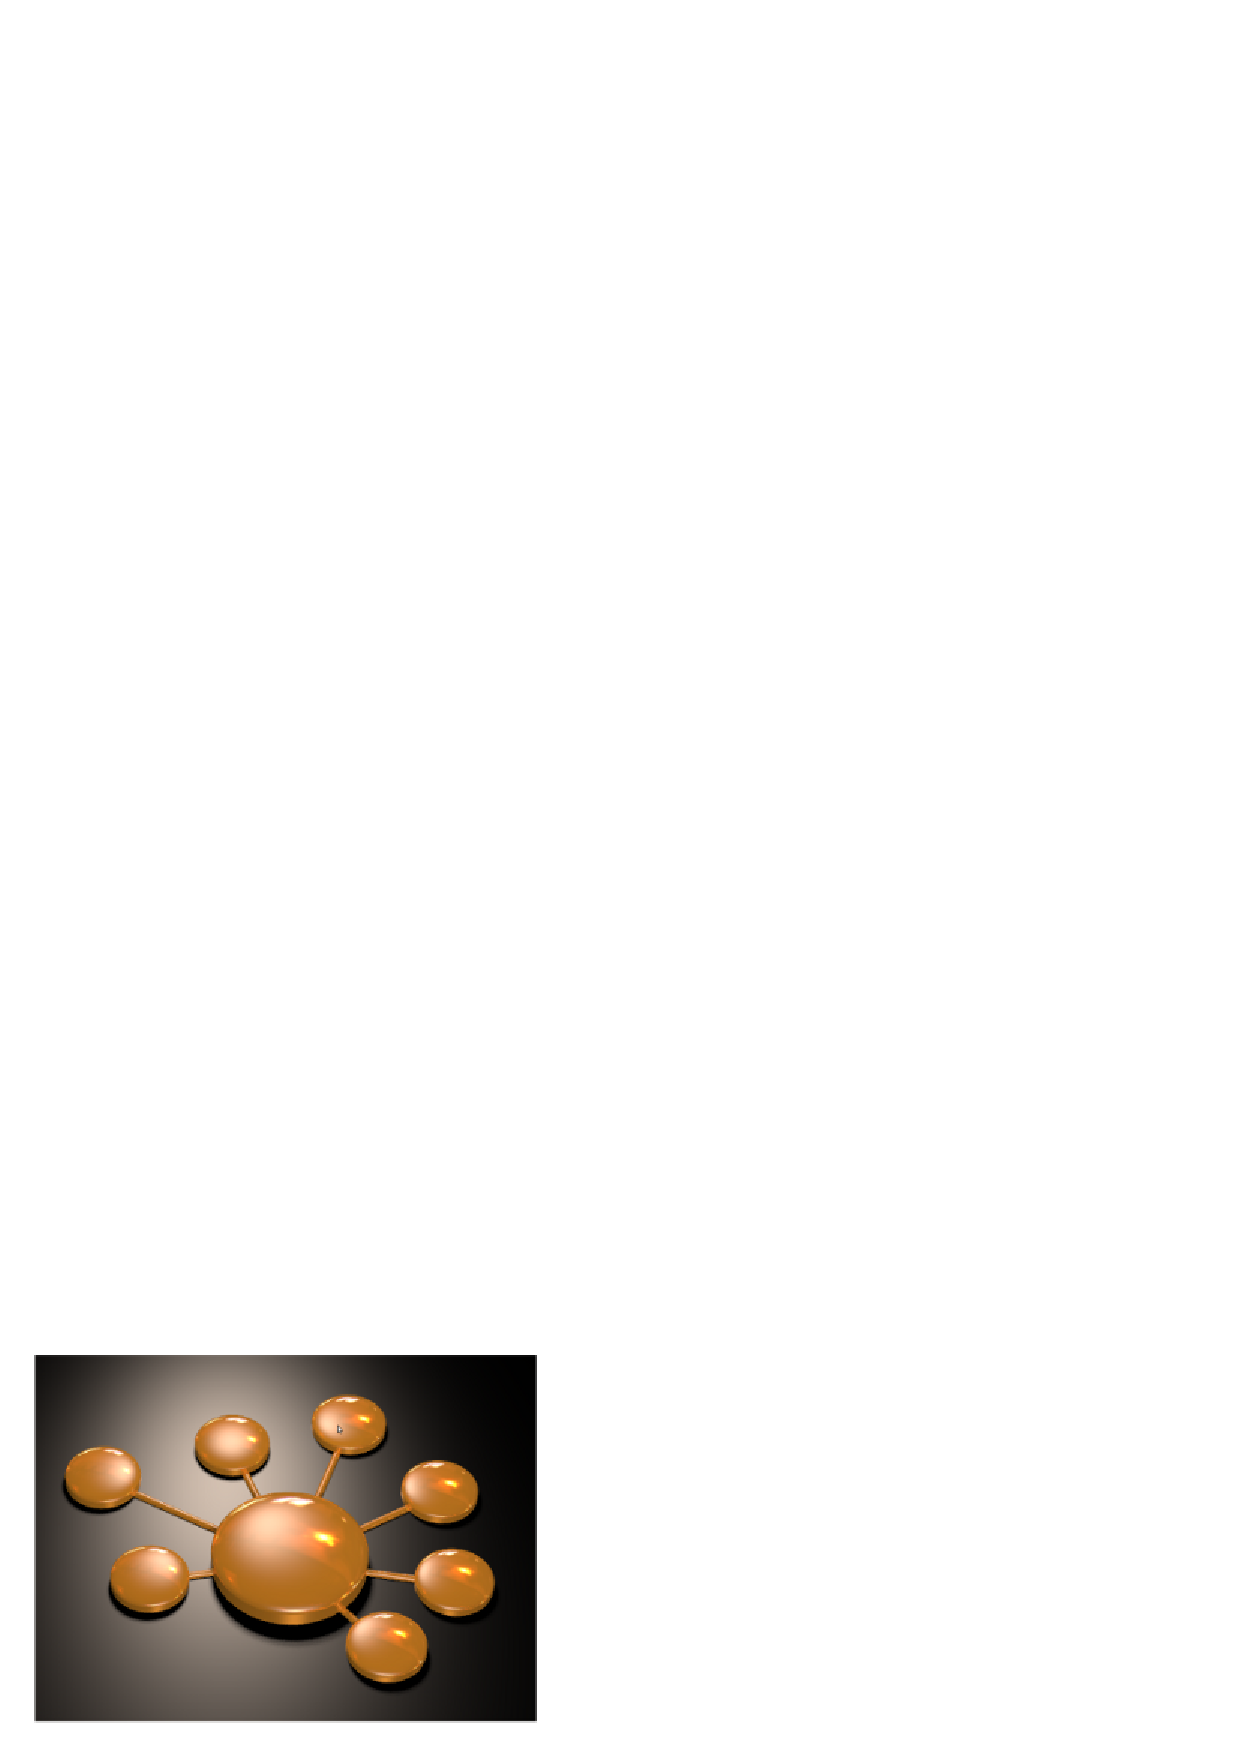
\includegraphics[scale=0.3]{SoFa_Logo}}}
\rput(-4,1.5){\href{http://www.sofa-framework.org/}{
		\begin{tabular}{l}
		\resizebox{4cm}{0.6cm}{SOFA} \\ 
		\resizebox{6cm}{0.3cm}{Simulation Open Framework Architecture}
		\end{tabular}
		}
	    }
\end{center}
%%%%%%%%%%%%%%%%%%   LOGO  %%%%%%%%%%%%%%%%%%%%%%%%%

%%%%%%%%%%%%%%%%%% DOCUMENT TITLE %%%%%%%%%%%%%%%%%%%%%%%%%
%\chapter{Mapping} %\section{Rigid Mapping} 
\vspace{1.5cm}
\begin{center}\resizebox{5cm}{0.6cm}{Rigid Mapping}\end{center}
%%%%%%%%%%%%%%%%%% DOCUMENT TITLE %%%%%%%%%%%%%%%%%%%%%%%%%

%%%%%%%%%%%%%%%%%%%%%%%%%%%%%%%%%%%%%%%%%%%%%%%%%%%%%%%%%%%%%%%%%%%%%%%%%%%%%%%%%%%%%%%%%
%=======================================================================================%
%%%%%%%%%%%%%%%%%%%%%%%%%%%%%%%%%%%%%%%%%%%%%%%%%%%%%%%%%%%%%%%%%%%%%%%%%%%%%%%%%%%%%%%%%
\paragraph{Motivation: } A rigid body (perfectly rigid) is an undeformable body. Computation for simulating its motion and colision is simpler than a deformable one. To optimize the computation, Rigid bodies in Sofa are presented by different models (Visual Model, Colision Model, Behaviour Model) ensuring their appropriate task. These model are related by the mapping (rigid mapping in this case).

%%%%%%%%%%%%%%%%%%%%%%%%%%%%%%%%%%%%%%%%%%%%%%%%%%%%%%%%%%%%%%%%%%%%%%%%%%%%%%%%%%%%%%%%%
%============================           FIGURE        ==================================%
\begin{figure}[h]
%\begin{center}
\begin{pspicture}(-7,-3)(7,3)
%\psline(-7,-3)(7,3)%%%%%%%%%%%%%%%%%%%%%%%%%%%%%
%%%%%%%%%%% Reference frame Observetor %%%%%%%%%%
\psline[linecolor=red]{->}(-3,-1.5)(-3,-0.5)%Z
\psline[linecolor=blue]{->}(-3,-1.5)(-2,-1.5)%Y
\psline[linecolor=green]{->}(-3,-1.5)(-3.3,-2.1)%X
\rput(-3.2,-1.5){O}
%%%%%%%%%%% Reference frame Rigid %%%%%%%%%%%%%%%
\psline[linecolor=red,linewidth=2pt]{->}(3.5,0.5)(4,0.7)%z
\psline[linecolor=blue,linewidth=2pt]{->}(3.5,0.5)(4.2,-0.2)%y
\psline[linecolor=green,linewidth=2pt]{->}(3.5,0.5)(4,1.5)%x
%%%%%%%%%%%%%%%%%%% Curve Rigid Surface %%%%%%%%%%%%%%%%%%%%%%%%%%%
\psccurve[showpoints=true](2.5,2)(2.5,-2)(4.5,-1)(6,2)%Pi P1 P2 P3
\rput(2.2,2.2){$P_i$}\rput(2.2,-2.2){$P_1$}\rput(4.8,-1){$P_2$}\rput(3.3,0.3){\textbf{P}$_0$}

\pnode(3.5,0.5){Po}\pnode(2.5,2){Pi}
\ncline[linestyle=dotted]{->}{Po}{Pi}\naput{$\vec{r}_i$}

\rput(-5,-1){\Rnode{Glob}{\Large{Global Frame}}}
\rput{30}(1,2){\Rnode{Loc}{\textbf{Local Frame}}}
\ncarc[arcangle=-40]{<->}{Loc}{Glob}\naput{Rotation}
%%%%%%%%%%%%%%%% Rotation axe %%%%%%%%%%%%%%%%%%%%%
\psline[linewidth=4pt]{->}(3.5,0.5)(7,0)%w(t) axe
\psellipticarc{<-}(5.5,0.25)(0.5,1){60}{320}
\rput(6,-0.2){w(t)}
\end{pspicture}
%\end{center}
\end{figure}
%============================           FIGURE        ==================================%
%%%%%%%%%%%%%%%%%%%%%%%%%%%%%%%%%%%%%%%%%%%%%%%%%%%%%%%%%%%%%%%%%%%%%%%%%%%%%%%%%%%%%%%%%
\paragraph{Definitions: }
\begin{itemize}
 \item Model Behaviour Rigid : Position and orientation (quaternion) of the center(s) of mass.
 \item Model Colision Rigid : A set of particles used for computing the colision with other objects.
 \item Model Visual Rigid : A set of particle used for visualizing.
\end{itemize}
Note that a rigid object can contain several rigid bodies (ex articulation system), consequently several center of mass. In the simple case, there is only one center. 
\paragraph{Computation: }By its proprety undeformable, rigid body composed a set of particles $P_i$ ensuring the distance of any pair of point and the angle of any pair of vectors remains constant in relation to time. Two frames of reference are needed to descript a rigid body : global and local. To find the position of any particles, only one particle is needed to be found in the global frames, then the other ones are related on the local frame. The center of mass is chosen naturally for the local frame origin $P_o$. After one step of time, the rigid position (linear and angular) can be changed. The mapping update all other particles potition and velocity knowing only these of the updated center. If the rigid is in colision, several particles are in solicitation. The mapping compute how are solicited the center of rigid. Assumed a rigid body has N particles : $P_{i\{i=0...N\}}$, their coordinates in the local frame are $r_i$. These works of mapping are descripted by those following algorithms :
\begin{center} To update the particles position :\end{center}
$
\left\|
  \begin{array}{lll}
  \text{Finding  } OP_o=LinearPosition; \\
  \text{Finding  } R^{glob}_{loc}=RotationMatrix; \\
  \text{For} (i=1;i<N;i++) \\
    \hspace{0.5cm} \{ \\
    \hspace{1cm} P_oP_i=R^{glob}_{loc}*r_i;\\
    \hspace{1cm} OP_i=OP_o+P_oP_i;\\
    \hspace{0.5cm} \} 
  \end{array}
\right.
$

\begin{center}To update the particles velocity : \end{center}
$
\left\|
  \begin{array}{lll}
  \text{Finding  } V_{P_O}=LinearVelocity; \\
  \text{Finding  } w_{Po}=AngularVelocity; \\
  \text{For} (i=1;i<N;i++) \\
    \hspace{0.5cm} \{ \\
    \hspace{1cm} V_i= V_{P_O} - P_oP_i \wedge w_{Po} ;\\
    \hspace{0.5cm} \} 
  \end{array}
\right.
$
\begin{center}To compute the external forces soliciting to center :  \end{center}    
$
\left\|
  \begin{array}{lll}
  \text{For} (i=1;i<N;i++) \\
    \hspace{0.5cm} \{ \\
    \hspace{1cm} F_{exter}+=f_i;\\
    \hspace{1cm} Torque+=P_oP_i  \wedge  f_i\\
    \hspace{0.5cm} \} \\
  \text{Update } LinearForce=F_{exter}; \\
  \text{Update } AngularForce=Torque; 
  \end{array}
\right.
$
\paragraph{Implementated code in Sofa: }These algorithms are implemented in Sofa by the following methods : \\
To update the particles position :
\begin{lstlisting}
template <class BasicMapping>
void RigidMapping<BasicMapping>::apply(typename Out::VecCoord& out, const typename In::VecCoord& in)
\end{lstlisting}
To update the particles velocity :
\begin{lstlisting}
template <class BasicMapping>
void RigidMapping<BasicMapping>::applyJ(typename Out::VecDeriv& out, const typename In::VecDeriv& in)
\end{lstlisting}
To compute the external forces soliciting to center :
\begin{lstlisting}
template <class BasicMapping>
void RigidMapping<BasicMapping>::applyJT(typename In::VecDeriv& out, const typename Out::VecDeriv& in)
\end{lstlisting}

\paragraph{Sofa Keyword: } MechanicalState, Bihaviour Model, Colision Model, Visual Model, Mapping, Quaternion. 


						      %%%%%%%%%%%%%%%%%%%%%%%%%%  Writer %%%%%%%%%%%%%%%%%%%%%%%%
						      \begin{flushright}
						      Document written by \\
						      \href{mailto:chi-thanh.nguyen@inria.fr}{{\textbf {Chi Thanh NGUYEN}}} \\
						      INRIA Lille
						      \end{flushright}
						      %%%%%%%%%%%%%%%%%%%%%%%%%%  Writer %%%%%%%%%%%%%%%%%%%%%%%%

\end{document}
